\documentclass{scrartcl}\usepackage[]{graphicx}\usepackage[]{color}
%% maxwidth is the original width if it is less than linewidth
%% otherwise use linewidth (to make sure the graphics do not exceed the margin)
\makeatletter
\def\maxwidth{ %
  \ifdim\Gin@nat@width>\linewidth
    \linewidth
  \else
    \Gin@nat@width
  \fi
}
\makeatother

\definecolor{fgcolor}{rgb}{0.345, 0.345, 0.345}
\newcommand{\hlnum}[1]{\textcolor[rgb]{0.686,0.059,0.569}{#1}}%
\newcommand{\hlstr}[1]{\textcolor[rgb]{0.192,0.494,0.8}{#1}}%
\newcommand{\hlcom}[1]{\textcolor[rgb]{0.678,0.584,0.686}{\textit{#1}}}%
\newcommand{\hlopt}[1]{\textcolor[rgb]{0,0,0}{#1}}%
\newcommand{\hlstd}[1]{\textcolor[rgb]{0.345,0.345,0.345}{#1}}%
\newcommand{\hlkwa}[1]{\textcolor[rgb]{0.161,0.373,0.58}{\textbf{#1}}}%
\newcommand{\hlkwb}[1]{\textcolor[rgb]{0.69,0.353,0.396}{#1}}%
\newcommand{\hlkwc}[1]{\textcolor[rgb]{0.333,0.667,0.333}{#1}}%
\newcommand{\hlkwd}[1]{\textcolor[rgb]{0.737,0.353,0.396}{\textbf{#1}}}%

\usepackage{framed}
\makeatletter
\newenvironment{kframe}{%
 \def\at@end@of@kframe{}%
 \ifinner\ifhmode%
  \def\at@end@of@kframe{\end{minipage}}%
  \begin{minipage}{\columnwidth}%
 \fi\fi%
 \def\FrameCommand##1{\hskip\@totalleftmargin \hskip-\fboxsep
 \colorbox{shadecolor}{##1}\hskip-\fboxsep
     % There is no \\@totalrightmargin, so:
     \hskip-\linewidth \hskip-\@totalleftmargin \hskip\columnwidth}%
 \MakeFramed {\advance\hsize-\width
   \@totalleftmargin\z@ \linewidth\hsize
   \@setminipage}}%
 {\par\unskip\endMakeFramed%
 \at@end@of@kframe}
\makeatother

\definecolor{shadecolor}{rgb}{.97, .97, .97}
\definecolor{messagecolor}{rgb}{0, 0, 0}
\definecolor{warningcolor}{rgb}{1, 0, 1}
\definecolor{errorcolor}{rgb}{1, 0, 0}
\newenvironment{knitrout}{}{} % an empty environment to be redefined in TeX

\usepackage{alltt}
\usepackage{tikz}
\usetikzlibrary{calc, shapes}
\usepackage{fp}
\usepackage{calc}
\usepackage{lmodern}
\usepackage{subcaption}
\usepackage[font=sf, labelfont={sf, bf}]{caption}
\usepackage{amssymb}
\usepackage{amsmath}
\usepackage{enumitem}
\usepackage{hyperref}
\usepackage[version=3,arrows=pgf-filled]{mhchem}
\usepackage{xspace}
\usepackage{multicol}
\usepackage{multirow}
\usepackage{lipsum}
\usepackage{csvsimple}
\usepackage{chemfig}
\usepackage{pgfplotstable}
\usepackage{longtable}
\usepackage{colortbl}
\usepackage{changes}

\pgfplotsset{compat=1.11}
% assign new commands
\newcommand{\degC}{\protect$\,^\circ$C\xspace}
\newcommand{\ul}{\protect\,$\mu$l\xspace}
\newcommand{\ug}{\protect\,$\mu$g\xspace}
\newcommand{\uM}{\protect\,$\mu$M\xspace}
\newcommand{\ra}{$\rightarrow$\xspace}

\newcommand{\od}{OD$^{600}$\xspace}
\newcommand{\odx}[1]{OD\(^{#1}\)\xspace}
% new commands end
\setlist{noitemsep}
\renewcommand*\printatom[1]{\ensuremath{\mathsf{#1}}}

%title etc
\author{Benjamin Weigel}
\title{WEB337 - \textit{in vivo} biotransformation}
\subtitle{using SOMT-2}
\date{\today}
\IfFileExists{upquote.sty}{\usepackage{upquote}}{}
\begin{document}
\sffamily
\maketitle

\tableofcontents
\listoffigures
\listoftables

\section{Introduction}

Test whether different substrates available in-lab are converted by SOMT-2 in vivo. Use SOMT seed culture to inoculate main cultures. Add substrates after 4 hours of incubation at 30\degC . 16 substrates means 16 flasks. Take two samples frome each flask at 0, 10, 20 and 30 hours. $16 \times 4 \times 2 = 128$ samples.
%\csvreader[tabular=llll,
%table head=No. & substrate & type & structure\\\hline,
%late after line=\\]%
%{RAW/substrates.csv}{no=\no, substrate=\substrate, type=\type, structure=\structure}%
%{\no & \substrate & \type & \tiny\structure}%

\section{Experimental}

\subsection{seed culture}
\begin{enumerate}[label=\arabic*)]
\item $\sim$10 mL pre-culture in LB supplemented with proper AB (100 ug/mL kanamycin)
\item grow over night at 30\degC and 220 rpm
\end{enumerate}

\subsection{main culture}

\begin{enumerate}[label=\arabic*)]
\item pellet cells (5 min @ 5000$\times g$, 4\degC) and wash with 15 mL PBS
\item resuspend pellet in the 3 mL of PBS
\item[\textbf{!!}]measure and record \od
\item inoculate 200 mL of autoinduction medium (+ 100 ug/mL kan) to an \od= 0.1
\item aliquot 10 mL into new flasks for each sample (17 flasks) (\emph{use 100 mL flasks})
\item add 0.1 mM of flavonoid (see \ref{sec:appendix}) from 10 mM stock in MeOH or DMSO to the cultures at 4 hours after inoculation (\od $\sim$ 0.8)
\vspace{0.5cm}
\item take a 600\ul sample at 10, 20 and 30 hours after inoculation and divide as follows: (\textbf{on ice!})
\begin{enumerate}[label=\alph*)]
\item measure \od ($\sim$100\ul)
\item 500\ul for HPLC (see \ref{sec:HPLC}) 
\end{enumerate}
\end{enumerate}

\subsection{\od measurements}
\begin{itemize}
\item[-]measure \od in MTP (all samples, 100\ul of sample) \textbf{!pathlength differs from cuvette!}
\item[-]measure \od of random samples in cuvette as reference
\end{itemize}

\subsection{HPLC}
\label{sec:HPLC}
\begin{enumerate}
\item extract 500\ul of culture \textbf{twice} with 500\ul ethyl acetate + 1\% formic acid
\item vortex for 30 s to extract, centrifgure for 10 min @ 10.000$\times g$, 4\degC to separate phases
\item pool organic phases and evaporate in SpeedVac (45\degC)
\item solve remainder in 200\ul MeOH
\item analyze via HPLC
\begin{description}
\item[Column:]
\item[Injection volume:] 10\ul
\item[Solvent A:] \cf{H2O} + 0.2\% formic acid
\item[Solvent B:] MeCN + 0.2\% formic acid
\item[Program:] 5\% B (hold 4 min) \ra 21 min ramp \ra 100\% B (hold 5 min)
\end{description}
\end{enumerate}

\section{Results}
\subsection{\od}

\begin{knitrout}
\definecolor{shadecolor}{rgb}{0.969, 0.969, 0.969}\color{fgcolor}\begin{figure}[]


{\centering 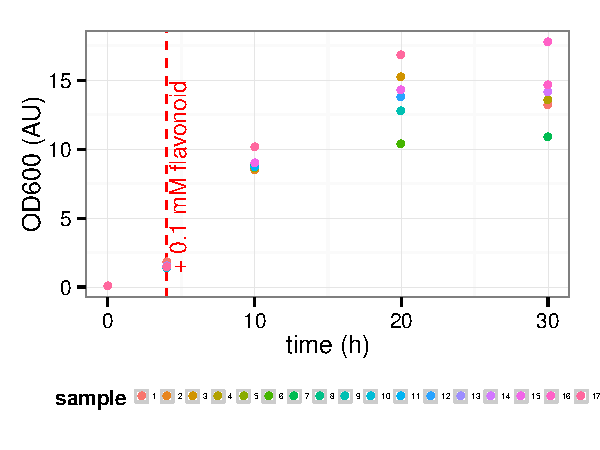
\includegraphics[width=\maxwidth]{figure/od-1} 

}

\caption[\od of samples]{\od of samples.\label{fig:od}}
\end{figure}


\end{knitrout}

\section{Appendix}
\label{sec:appendix}
\pgfplotstabletypeset[
    col sep=comma,
    begin table=\begin{longtable},
    end table=\end{longtable},
    string type,
	every head row/.append style={
		after row={%
			\hline\endhead
		},
		before row={%
			\hline
		}
	},
	every even row/.style={before row={\rowcolor[gray]{0.9}}},
    every last row/.style={after row=\hline},
    columns/no/.style={column name=No., column type=l},
    columns/substrate/.style={column name=substrate, column type=l},
    columns/type/.style={column name=moiety, column type=l},
    columns/structure/.style={
    	column name=structure, 
    	column type=c,
		postproc cell content/.append style={
			/pgfplots/table/@cell content/.add={\tiny}{},
		},    	
    },
    ]{RAW/substrates.csv}



\end{document}
